\documentclass[abstract=on,9pt,twocolumn]{scrartcl}

\usepackage[utf8x]{inputenc}
\usepackage[T1]{fontenc}
\usepackage[english]{babel}

\usepackage{graphicx}%	images other than eps

% \usepackage[paper=a4paper,top=2cm,left=1.5cm,right=1.5cm,bottom=2cm,foot=1cm]{geometry}

%	relative font sizes
\usepackage{relsize}

% \usepackage[retainorgcmds]{IEEEtrantools}%	IEEEeqnarray
% \setlength{\IEEEnormaljot}{4\IEEEnormaljot}

% \usepackage{graphicx}
% \usepackage{epstopdf}
% \usepackage{indentfirst}
\usepackage{hyperref}
\usepackage{cleveref}
% %\usepackage[noabbrev]{cleveref}
% \usepackage{listings}
% \usepackage{color}


\graphicspath{{../images/}}

%	TODO assignments and notes
\usepackage{todonotes}
\newcommand{\todoline}[2][inline]{\todo[#1]{#2}}

\newcommand{\todopfac}[1]{\todo[inline,color=red!40]{#1}}
\newcommand{\todonaps}[1]{\todo[inline,color=green!40]{#1}}

\usepackage{xspace}
\newcommand{\treetiler}{\textit{TreeTiler}\xspace}

% %%%%%%%%%%%
% %  Hacks  %
% %%%%%%%%%%%

% %	Paragraph (title) with linebreak
% \newcommand{\paragraphh}[1]{\paragraph{#1\hfill}\hfill

% }

%	Add "Appendix" to the appendices titles, but not to the references
\usepackage{ifthen}
\newcommand*{\appendixmore}{%
  \renewcommand*{\othersectionlevelsformat}[1]{%
    \ifthenelse{\equal{##1}{section}}{\appendixname~}{}%
    \csname the##1\endcsname\autodot\enskip}
  \renewcommand*{\sectionmarkformat}{%
    \appendixname~\thesection\autodot\enskip}
}


% Title page

% Minho
% \titlehead{University of Minho \hfill Master's Degree in Informatics Engineering\\	Department of Informatics \hfill Parallel and Distributed Computing}

% Texas
\titlehead{University of Texas%
%\hfill Summer Internship\\%
\\%
\hfill Institute for Computational Engineering and Sciences%
\hfill Center for Distributed and Grid Computing}

%\title{TreeTiler Optimization Techniques applied to the Galois System}
\title{Improving Locality on Traversal of Recursive Structures}

% kind of unecessary i think
%\subtitle{Manual approach}

\author{Miguel~Palhas\\\texttt{\smaller mpalhas@ices.utexas.edu}%
\and Pedro~Costa\\\texttt{\smaller pcosta@ices.utexas.edu}%\\
%\smaller Stéphane Clain (co-Advisor)\\
% Pingali
% Andrew
% Donald
}

\date{Austin, Texas, U.S.A. --- August 2012}

\subject{Summer Internship}

\begin{document}
\maketitle

\begin{abstract}
Locality in algorithms using irregular structures is naturally difficult to improve. This document reviews a new approach to these algorithms in the form of two optimizations, which change how the structures are traversed. Three implementations of example algorithms are also described in this document: Barnes-Hut, Point Correlation and Ray Tracing. These examples are parallelized using the Galois framework. Measurements showed that only the first two examples got speedups, but all reduced cache miss rates considerably for the first two levels.
\end{abstract}	% Abstract
\section{Introduction}
\label{sec:intro}

This document follows the work described in \cite{tree_tiler}, where a framework called TreeTiler is presented, to optimize, at both compile time and run time, locality of algorithms relying on the traversal of recursive data structures.

In the following sections, the optimizations implemented in the TreeTiler framework are reviewed and applied to three test cases. These cases were selected to match the experiences performed in \cite{tree_tiler} and use the Galois framework\cite{galois} for parallelization. The goal of this document is to study the impact of these optimizations along with Galois.

\Cref{sec:tiler} explains the original work and the \treetiler framework, with a particular focus on the implemented optimizations in \cref{sec:optim}. In \cref{sec:cases} the implemented test cases and each of their particularities are explained. Measurement results are all presented in \cref{sec:results} with some final considerations and conclusions in \cref{sec:conclusion}. \Cref{sec:env} detail the testing environment used to achieve the results shown.		% Introduction
\section{TreeTiler}
\label{sec:tiler}

The work showed on \cite{tree_tiler} presents a framework, \treetiler, that can be used to refactor Java code at runtime. Given a Java application source code as input, \treetiler will try to detect a recursive data structure. It will then look for a recursive method that performs a recursive traversal on that structure.

The JastAdd framework is employed to analyse and refactor the Java input at compile time, generating the output consisting of the same program with the applied optimizations, which are described here.

\subsection{Optimizations}
\label{sec:optim}

The techniques employed by \treetiler deal with the way a recursive structure is traversed. Even though it is commonly an irregular structure, some techniques can be applied to exploit locality when multiple traversals are done. In this report, the techniques used were the Spatial Sort and Point Blocking. An Auto Tuner is also added to the Java code by \treetiler. This Tuner tries to find the best parameters for the optimizations, which sometimes are input dependent and cannot be evaluated at compile time.

\subsubsection{Sorting}
\label{sec:optim:sort}

Traversing an irregular structure requires loading from memory the elements of the structure which, due to their irregular nature, can not be obtained in an optimized way through prefetching. Also, the elements of this structure which are consecutively accessed (especially in parallel) will most probably lie in distinct cache lines, hurting locality.

By changing the order of accesses in these structures, so that domain objects with similar traversal patterns become consecutive, temporal locality is improved as the elements a given object will touch are already likely to have been touched by the previous one.

Sorting these objects in applications where the domain refers to a notion of space can be performed using space-filling curves\footnote{A curve which touches every object in the domain only once. Examples of these curves are the Peano and Hilbert curves.} (for algorithms in the space domain like Barnes-hut). The examples described in this document use the CGAL library, implementing the traits required for spatial sorting in 3D.

\begin{figure}[!htp]
	\centering
	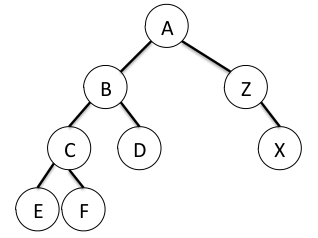
\includegraphics[width=0.4\columnwidth]{pointblocking_tree}
	\caption{A sample tree}
	\label{fig:tree}
\end{figure}

\begin{figure}[!htp]
	\centering
	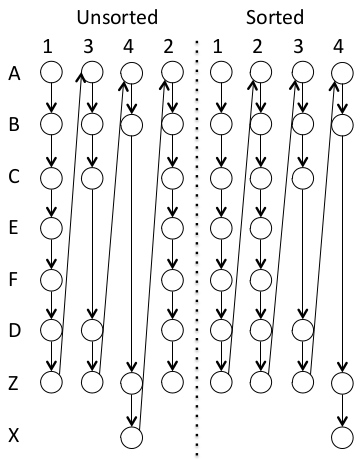
\includegraphics[width=0.6\columnwidth]{pointblocking_sort}
	\caption{Spatial Sort transformation applied to traversal of tree shown in \cref{fig:tree}}
	\label{fig:sort}
\end{figure}

\paragraph{Limitations:}
Processing objects in an order which brings similar traversals closer in time only brings improvements when the traversal itself fits in cache. This will allow subsequent objects to take advantage of the acceleration structure elements already visited by previous objects. For sufficiently deep traversals, when the subsequent objects traverse the structure, the first elements have already been evicted from cache. \cite{tree_tiler} already shows that as the traversal size increases, the locality improvements gained from the Sorting optimization decrease drastically.

\subsubsection{Blocking}
\label{sec:optim:block}

Since it is likely that geometrically closer points also follow a similar traversal, which is the basis for the Spatial Sort optimization, it is also likely that those points can be processed in blocks, rather than one at a time, thus taking advantage of locality, and preventing the traversal from being evicted too soon from cache.

Instead of traversing the structure for a single point, and iteratively switching points, the new strategy takes advantage of the premise that Spatial Sort rearranges points so that a small subset of points is likely to be geometrically close to each other. This subset is grouped into a block, and the tree is traversed for that block at the same time.

The root node of the structure is processed for all points of the block. If necessary (depending on the algorithm), if the paths of each point in the block diverge at a given node, it may be necessary to split the block into smaller blocks, each one going to a different node. Given the geometrical proximity, this is only more likely to occur at the last levels of the structure, allowing for some locality to still be gained in the previous levels.

\Cref{fig:sort} illustrates the execution order of a point blocked implementation, compared to the non blocked, sorted implementation.

\begin{figure}[!htp]
	\centering
	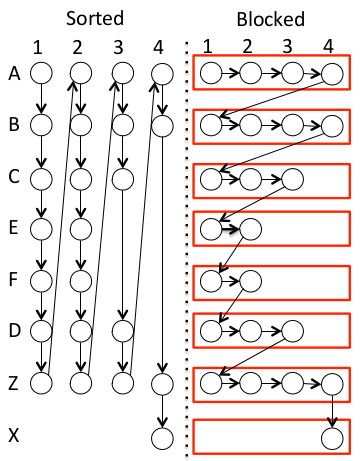
\includegraphics[width=0.6\columnwidth]{pointblocking_blocks}
	\caption{Point Blocking transformation}
	\label{fig:sort}
\end{figure}

It is intuitive to notice that this strategy is only good if the points within a block are likely to follow a similar traversal path, otherwise too much divergence will hinder performance much like the original strategy.

\subsubsection{Auto Tuner}
\label{sec:optim:tuner}
The optimal block size is dependent on both hardware and algorithm details, but it may also be input dependent. The optimal block size for a Barnes-Hut implementation might not be the same as the ideal block size for a Ray Tracing application. Given that, a generic framework like \treetiler must not make assumptions about the algorithm and the input only at compile time.

For that reason, \treetiler installs an AutoTuner in the output code. This AutoTuner will perform a small sample (possibly selected randomly) of block iterations, and evaluate their performance at runtime.
Tipically, it is expected that a block size too small will yield bad results, possibly even worse than the original version, due to large overhead of the additional instructions for the point blocking, and because of the fact that misses in the tree occur between each block. In contrast, a block size too big wil not fit in cache, and misses will occur in the block items instead.

A sweet spot is expected to occur where the block size is near ideal value, meaning the block size is large enough to avoid cache misses in the tree, but still small enough to fit in cache.

The AutoTuner might then start at a small block size, and process the chosen samples, measuring the average traversal time for each subsequent block size. The time is expected to reduce until the sweet spot is reached, at which point the time will start to increase again.
When this happens, the best block size is the one that yielded the lowest runtime.
	% TreeTiler
\section{Study Cases}
\label{sec:cases}

The studied optimizations, previously described in \cref{sec:optim} were applied to three different algorithms. The work focused mostly on the Spatial Sort and Point Blocking techniques. AutoTuner was not implemented, as this was not a generic framework like \treetiler, and as such there was no need for a tool to automatically determine the ideal parameters. The implemented test cases were:

\begin{description}
	\item[\textbf{Barnes-Hut}]
		This was the first test case, based on the implementation provided on the sample applications from the Galois framework. The acceleration structure used here was the already provided Octree.

	\item[\textbf{Point Correlation}]
		Implemented from scratch. In terms of implementation, it is mostly equivalent to that of the Barnes-Hut example, with the biggest difference being in the acceleration structure used, which is a KD-Tree rather than an Octree,

	\item[\textbf{Ray Tracer}]
		Based on a simple unoptimized implementation in OpenMP. A Bounding Volume Hierarchy implementation was designed for the acceleration structure.
\end{description}

\Cref{sec:cases:barnes,sec:cases:pointcorr,sec:cases:ray} explain with some more detail each test case.

\subsection{barneshut}
\label{sec:cases:barnes}

\todoline{THIS}
For the first test case, the Barnes-Hut implementation provided in the sample applications of the Galois framework was used.
This original implementation used an Octree as the acceleration structure, and served as a starting point to the usage of the Galois framework. Only the optimizations were left to implement.
\subsection{Two Point Correlation}
\label{sec:cases:pointcorr}

\todopfac{THIS}
\subsection{Ray Tracer}
\label{sec:cases:ray}

\todonaps{THIS}		% Study Cases
\section{Results}
\label{sec:results}

\todopfac{THIS}		% Comparison results
\section{Conclusions}
\label{sec:conclusion}

In this document, two optimizations performed by the \treetiler framework to increase locality in irregular applications with acceleration structures were reviewed and applied to three distinct examples (Barnes-hut, Two Point Correlation and a Ray Tracer) using the Galois framework.

The first optimization consisted in sorting the domain objects in such a way that similar patterns traversing the acceleration structure would be processed consecutively. This allows an increase in temporal locality, but fails when the traversal is too deep to fit in cache.

Blocking (the second optimization) applies a tilling approach to group objects during the traversal of the tree. Applied together with Sorting this amplifies temporal locality, allowing multiple objects with similar patterns to traverse the tree together, thus decreasing cache misses for each level of the acceleration structure.

For Barnes-hut, Galois already presented a functional implementation, using an Octree. The implementation of the Sorting optimization was performed using the CGAL library to spatially sort the bodies. Blocking required a change in the Octree traversal so that groups of bodies would be considered together for each node.

The Two Point Correlation example was implemented entirely from scratch using a kD-Tree as an acceleration structure. Also being an N-Body problem, it differs from the Barnes-hut example in both the acceleration structure and the need for a reduction to compute the final result in a parallel execution. Despite that, the implementation of both optimizations is similar.

As for the Ray Tracer, an implementation already available online was used as the base. The final implementation processes one pixel at a time parallelizing the computation of the rays. Due to the increased complexity of this problem, where both the origin and the direction of the rays must be taken into account for Sorting, rays are resorted and blocks rebuilt after each level of rays has been computed.

Results showed significant improvements in speedups due to the decrease of cache misses in both Barnes-hut and the Two Point Correlation example. While improvements regarding cache misses also exist in the Ray Tracer example, the highly divergent characteristics of the algorithm make the management of the blocks too costfull for any speedups to exist.

Proven the effects of the described optimizations in the temporal locality of irregular structures, future work can focus in implementing a generic way for Galois to apply these optimizations at compile time, as described in the \treetiler framework. After this, an automatic tuning tool similar to the AutoTuner in \treetiler could be implemented to optimize the parameters for a given implementation in runtime.	% Conclusion

\bibliographystyle{IEEE}
\bibliography{report}

\appendix

\section{Environmental Setup}
\label[appendix]{sec:env}

All the results retrieved for this document were obtained using tests performed in the Maxwell machine\footnote{\ttfamily maxwell.ices.utexas.edu}. \Cref{tab:maxwell} shows the hardware description of this machine.

\begin{table}[!htp]
	\begin{center}
		\begin{tabular}{rl}
			\hline
			Processors: & 4	\\
			Processor model: & \intel\xeon X5570	\\
			Cores per processor: & 6	\\
			Threads per core: & 2	\\
			Clock frequency: & 2.93 GHz	\\
			\hline
			L1 cache: & 32 KB + 32 KB per core	\\
			L2 cache: & 256 KB per core	\\
			L3 cache: & 8 MB shared	\\
			RAM: & 23 GB	\\
			\hline
		\end{tabular}
		\caption[Maxwell machine hardware description.]{Maxwell machine hardware description. See \cite{xeon5500} for further detail about this processor.}
		\label{tab:maxwell}
	\end{center}
\end{table}		% Environmental Setup
\section{Methodology}
\label{sec:method}	% Methodology

\end{document}
